\documentclass[aspectratio=169,11pt]{beamer}

\usepackage{beamerthememinimal}
\usepackage{tikz}
\usetikzlibrary{shapes.geometric, arrows.meta, positioning, calc}
\usepackage{booktabs}
\usepackage{graphicx}
\usepackage{amsmath,amssymb}
\usepackage{hyperref}

% Auto-generated macros from metrics JSON
\newcommand{\dimXTwoD}{2}
\newcommand{\dimYTwoD}{4}
\newcommand{\numTransformsTwoD}{6}
\newcommand{\numBinsTwoD}{8}
\newcommand{\hiddenDimTwoD}{128}
\newcommand{\contextHiddenTwoD}{64}
\newcommand{\dimXSixD}{6}
\newcommand{\dimYSixD}{8}
\newcommand{\numTransformsSixD}{8}
\newcommand{\numBinsSixD}{10}
\newcommand{\hiddenDimSixD}{256}
\newcommand{\contextHiddenSixD}{128}
\newcommand{\pairAUCTwoD}{0.4231}
\newcommand{\pairAUCStdTwoD}{0.0109}
\newcommand{\nullThreshTwoD}{0.5244}
\newcommand{\controlAUCTwoD}{0.8277}
\newcommand{\pairAUCSixD}{0.4502}
\newcommand{\pairAUCStdSixD}{0.0192}
\newcommand{\nullThreshSixD}{0.5274}
\newcommand{\controlAUCSixD}{0.8973}


\title[cINN Detector Unfolding]{\textbf{Unbinned Multidimensional Detector Unfolding\\with Conditional Invertible Neural Networks (cINNs)}}
\subtitle{OmniFold $Z+\text{jets}$ Benchmark on Delphes Fast Simulation}
\author[Alfien \& Boopesh]{%
  \textbf{Alfien Jessurun P} (ep23btech11001) \quad \& \quad \textbf{Boopesh D} (ep23btech11007)%
}
\institute[IIT Hyderabad]{%
  Department of Physics\\
  \textbf{Indian Institute of Technology Hyderabad}%
}
\date{\today}

\begin{document}

% -------------------------------------------------------------
% Slide 1: Title Frame
% -------------------------------------------------------------
\begin{frame}
  \titlepage
  \note{Welcome everyone. Today we present our work on unbinned multidimensional detector unfolding using Conditional Invertible Neural Networks (cINNs), applied to the LHC Z+jets Delphes benchmark. This project was conducted by Alfien Jessurun and Boopesh D at IIT Hyderabad.}
\end{frame}

% -------------------------------------------------------------
% Slide 2: Problem and Approach
% -------------------------------------------------------------
\begin{frame}{1. Problem Statement: The Detector Inverse Problem}
  \begin{columns}[T]
    \begin{column}{0.58\textwidth}
      \begin{itemize}
        \item \textbf{Particle Level ($x \in \mathbb{R}^D$):} True hadronization states from QCD theory.
        \item \textbf{Detector Level ($y \in \mathbb{R}^M$):} Distorted by smearing, resolution, and cuts.
        \item \textbf{The Inverse Challenge:} Reconstructing continuous $p(x_{\text{gen}} \mid y_{\text{sim}})$.
        \item \textbf{Curse of Binned Unfolding (IBU):} $B^D$ bins scale exponentially (in 6D: $20^6 = 6.4 \times 10^7$ cause bins).
        \item \textbf{cINN Solution:} Continuous, unbinned, event-by-event sampling via normalizing flows.
        \item \textbf{Benchmark Data:} $pp \to Z+\text{jets}$ at $\sqrt{s}=14$ TeV (Pythia26 train, Herwig held out).
      \end{itemize}
    \end{column}
    \begin{column}{0.38\textwidth}
      \centering
      \vspace{0.2cm}
      \fbox{\parbox[c][3.8cm][c]{4.6cm}{\centering \footnotesize \textbf{Context: LHC CMS Detector}\\Particle collisions produce high-$p_T$ jets distorted by calorimeter resolution.\\\vspace{0.2cm}\tiny [Source: CERN CMS Collaboration]}}
      \vspace{0.1cm}
      \tiny\textit{Inversion requires learning full multi-differential distributions.}
    \end{column}
  \end{columns}
  \note{In experimental particle physics, detectors introduce resolution smearing, tracking inefficiencies, and acceptance losses. Traditional Iterative Bayesian Unfolding requires discretizing observables into histogram bins, which scales exponentially as B to the power D, causing memory explosion in higher dimensions. We resolve this by training a conditional invertible neural network that directly models the continuous posterior density of true particles conditioned on detector measurements.}
\end{frame}

% -------------------------------------------------------------
% Slide 3: cINN Architecture (Overview)
% -------------------------------------------------------------
\begin{frame}{2. cINN Architecture: Global System Overview}
  \centering
  \begin{tikzpicture}[scale=0.88, every node/.style={transform shape}]
    % Detector conditioning path
    \node[draw, rounded corners, fill=IITHorange!15, text width=2.4cm, align=center, font=\small] (reco) at (0, 2.5) {Reco Jet $y$\\($M$-dim)};
    \node[draw, rounded corners, fill=IITHyellow!30, text width=3.2cm, align=center, font=\small, right=0.9cm of reco] (mlp) {Context Embedding\\$h(y) \in \mathbb{R}^{C}$};
    
    % Flow chain
    \node[draw, rounded corners, fill=green!15, text width=2.0cm, align=center, font=\small] (truth) at (0, 0) {Gen Jet $x$\\($D$-dim)};
    \node[draw, fill=IITHorange!20, text width=1.6cm, align=center, font=\small, right=0.8cm of truth] (b1) {RQ-Spline\\Block 1};
    \node[font=\large, right=0.4cm of b1] (dots) {$\cdots$};
    \node[draw, fill=IITHorange!20, text width=1.6cm, align=center, font=\small, right=0.4cm of dots] (bk) {RQ-Spline\\Block $K$};
    \node[draw, rounded corners, fill=purple!15, text width=2.2cm, align=center, font=\small, right=0.8cm of bk] (latent) {Latent $z$\\$\sim \mathcal{N}(0, I_D)$};

    % Arrows
    \draw[-{Stealth[scale=1.1]}, thick] (reco) -- (mlp);
    \draw[-{Stealth[scale=1.1]}, thick] (truth) -- (b1);
    \draw[-{Stealth[scale=1.1]}, thick] (b1) -- (dots);
    \draw[-{Stealth[scale=1.1]}, thick] (dots) -- (bk);
    \draw[-{Stealth[scale=1.1]}, thick] (bk) -- (latent);

    % Context conditioning lines
    \draw[-{Stealth[scale=1.1]}, dashed, thick, IITHorange] (mlp.south) |- (b1.north);
    \draw[-{Stealth[scale=1.1]}, dashed, thick, IITHorange] (mlp.south) |- (bk.north);

    % Bidirectional annotation
    \node[font=\footnotesize, text=IITHdark] at (5.2, -1.0) {\textbf{Forward (Encoding / Train):} $x \to z$ with exact Jacobian determinant};
    \node[font=\footnotesize, text=IITHdark] at (5.2, -1.4) {\textbf{Inverse (Unfolding / Sample):} Draw $z \sim \mathcal{N}(0, I_D)$, invert $f^{-1}(z; h(y)) \to x_{\text{unf}}$};
  \end{tikzpicture}
  \note{Here is the global architecture. Reconstructed detector observables y pass through a feed-forward context embedding MLP to extract conditioning representations. In the forward pass during training, true particle observables x pass through a chain of K invertible spline blocks, mapping into an isotropic Gaussian latent space. During inference, we draw random noise from the Gaussian and evaluate the exact analytical inverse conditioned on y to obtain unfolded physics events in milliseconds.}
\end{frame}

% -------------------------------------------------------------
% Slide 4: Substructure of One RQ-Spline Block
% -------------------------------------------------------------
\begin{frame}{3. Substructure: Conditional RQ-Spline Coupling}
  \begin{columns}[T]
    \begin{column}{0.50\textwidth}
      \centering
      \begin{tikzpicture}[scale=0.78, every node/.style={transform shape}]
        \node[draw, fill=lightgray!30, font=\scriptsize] (u) at (0, 3.5) {Input $[u_1, u_2]$};
        \node[draw, fill=IITHyellow!30, font=\scriptsize] (ctx) at (2.4, 3.5) {Context $c$};
        
        \node[draw, rounded corners, fill=IITHorange!20, text width=2.4cm, align=center, font=\scriptsize] (cond) at (1.5, 2.0) {Conditioner MLP\\$[u_1, c] \to \text{Knots}$};
        \node[draw, rounded corners, fill=green!20, text width=2.8cm, align=center, font=\scriptsize] (spline) at (1.5, 0.6) {Rational-Quadratic\\Spline Transform};
        \node[draw, fill=lightgray!30, font=\scriptsize] (v) at (0, -0.6) {Output $[u_1, v_2]$};

        \draw[->, thick] (u) -| (cond);
        \draw[->, thick] (ctx) -- (cond);
        \draw[->, thick] (cond) -- (spline);
        \draw[->, thick] (u) |- (spline);
        \draw[->, thick] (spline) -| (v);
      \end{tikzpicture}
    \end{column}
    \begin{column}{0.48\textwidth}
      \begin{table}[htbp]
\centering
\footnotesize
\begin{tabular}{lcc}
\toprule
\textbf{Hyperparameter} & \textbf{2D Target ($m, M$)} & \textbf{6D Target (Full OmniFold)} \\
\midrule
Target observables ($x$) & 2 ($m$, Multiplicity) & 6 ($m, M, w, m_{SD}, z_g, \tau_2$) \\
Conditioning inputs ($y$) & 4 ($m, M, p_T, \eta$) & 8 ($m, M, w, m_{SD}, z_g, \tau_2, p_T, \eta$) \\
RQ-Spline Transforms ($K$) & 6 & 8 \\
Spline Bins ($K_b$) & 8 & 10 \\
Conditioner MLP Hidden & 3 layers $\times$ 128 & 3 layers $\times$ 256 \\
Context Embedding $h(y)$ & 4 $\to$ 64 $\to$ 64 & 8 $\to$ 128 $\to$ 128 \\
Feature Permutation & Reverse alternate & Alternating forward/reverse \\
\bottomrule
\end{tabular}
\end{table}

      \vspace{0.1cm}
      \tiny\textit{Alternating autoregressive permutations ensure full feature mixing.}
    \end{column}
  \end{columns}
  \note{Looking inside each block, we utilize monotonic rational-quadratic splines from the Zuko library. Within each of the bins, the transformation is a quotient of two quadratic polynomials. Conditioners take the untouched coordinates and context to output bin widths, heights, and derivatives. As shown in the table, our 2D model uses 6 transforms with 8 bins, while the 6D model scales to 8 transforms with 10 bins and 256 hidden channels.}
\end{frame}

% -------------------------------------------------------------
% Slide 5: Preprocessing and Training Pipeline
% -------------------------------------------------------------
\begin{frame}{4. Preprocessing and Training Engine}
  \begin{columns}[T]
    \begin{column}{0.55\textwidth}
      \begin{itemize}
        \item \textbf{Invertible Pipeline ($x \leftrightarrow u$):}
          \begin{itemize}\footnotesize
            \item Heavy-tailed ($m, m_{\text{SD}}$): $u = \log(x + \epsilon)$
            \item Bounded ($w, \tau_2 \in [0, 1]$): scaled logit mapping
            \item Discrete multiplicity ($M \in \mathbb{Z}^+$): uniform dequantization $U(0, 1)$
            \item Zero spike ($z_g = 0$): zero-inflated training noise
          \end{itemize}
        \item \textbf{Leakage Protection:} Standardized strictly on Pythia train.
        \item \textbf{Optimization:} AdamW ($\eta = 10^{-3}$), Cosine Annealing, patience = 10 epochs over 3 independent seeds.
      \end{itemize}
    \end{column}
    \begin{column}{0.43\textwidth}
      \begin{block}{Exact Negative Log-Likelihood}
        \centering
        \vspace{0.1cm}
        
\includegraphics[width=0.92\textwidth]{images/equations/eq_nll.png}
        \vspace{0.1cm}
      \end{block}
      \vspace{0.2cm}
      \begin{itemize}\footnotesize
        \item Closed-form Jacobian log-determinant.
        \item Verified against PyTorch autograd.
        \item Fast, stable convergence on RTX 5070 Ti.
      \end{itemize}
    \end{column}
  \end{columns}
  \note{Because particle physics observables carry physical boundaries such as non-negative masses and discrete particle counts, feeding them raw causes boundary distortion. We constructed a strictly invertible preprocessing pipeline with exact analytical Jacobians: log transforms for heavy tails, logit for bounded shapes, and dequantization noise for integer multiplicities. Training minimizes the exact negative log likelihood with early stopping across three seeds.}
\end{frame}

% -------------------------------------------------------------
% Slide 6: Distribution Agreement Metrics
% -------------------------------------------------------------
\begin{frame}{5. Metrics (1/2): Physics Marginals \& Distances}
  \begin{columns}[T]
    \begin{column}{0.48\textwidth}
      \begin{itemize}
        \item \textbf{Wasserstein-1 Distance ($W_1$):}
          \vspace{0.1cm}\\
          \centering
          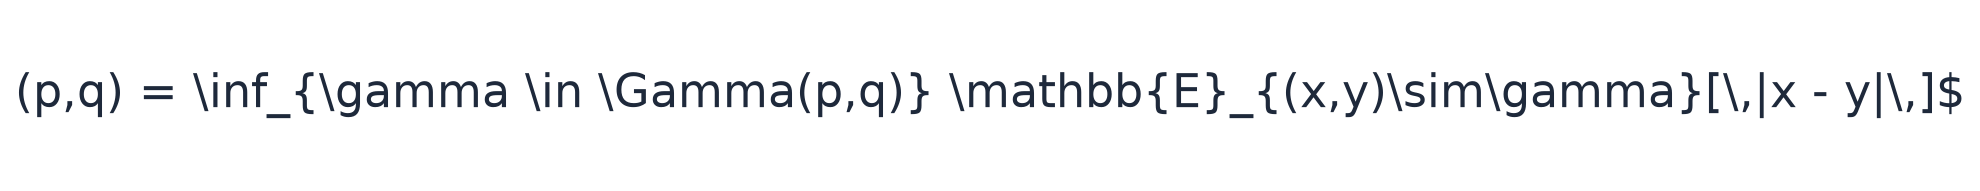
\includegraphics[width=0.92\textwidth]{images/equations/eq_w1.png}\\
          \vspace{0.1cm}
          \raggedright
          \footnotesize Physical transport cost in GeV / counts.
        \item \textbf{Kolmogorov-Smirnov (KS):}
          Max eCDF distance across observables.
        \item \textbf{Binned $\chi^2 / \text{ndf}$:} Local bin-by-bin test.
        \item \textbf{Performance:} cINN reduces mass $W_1$ by $>90\%$ compared to raw detector reco.
      \end{itemize}
    \end{column}
    \begin{column}{0.50\textwidth}
      \centering
      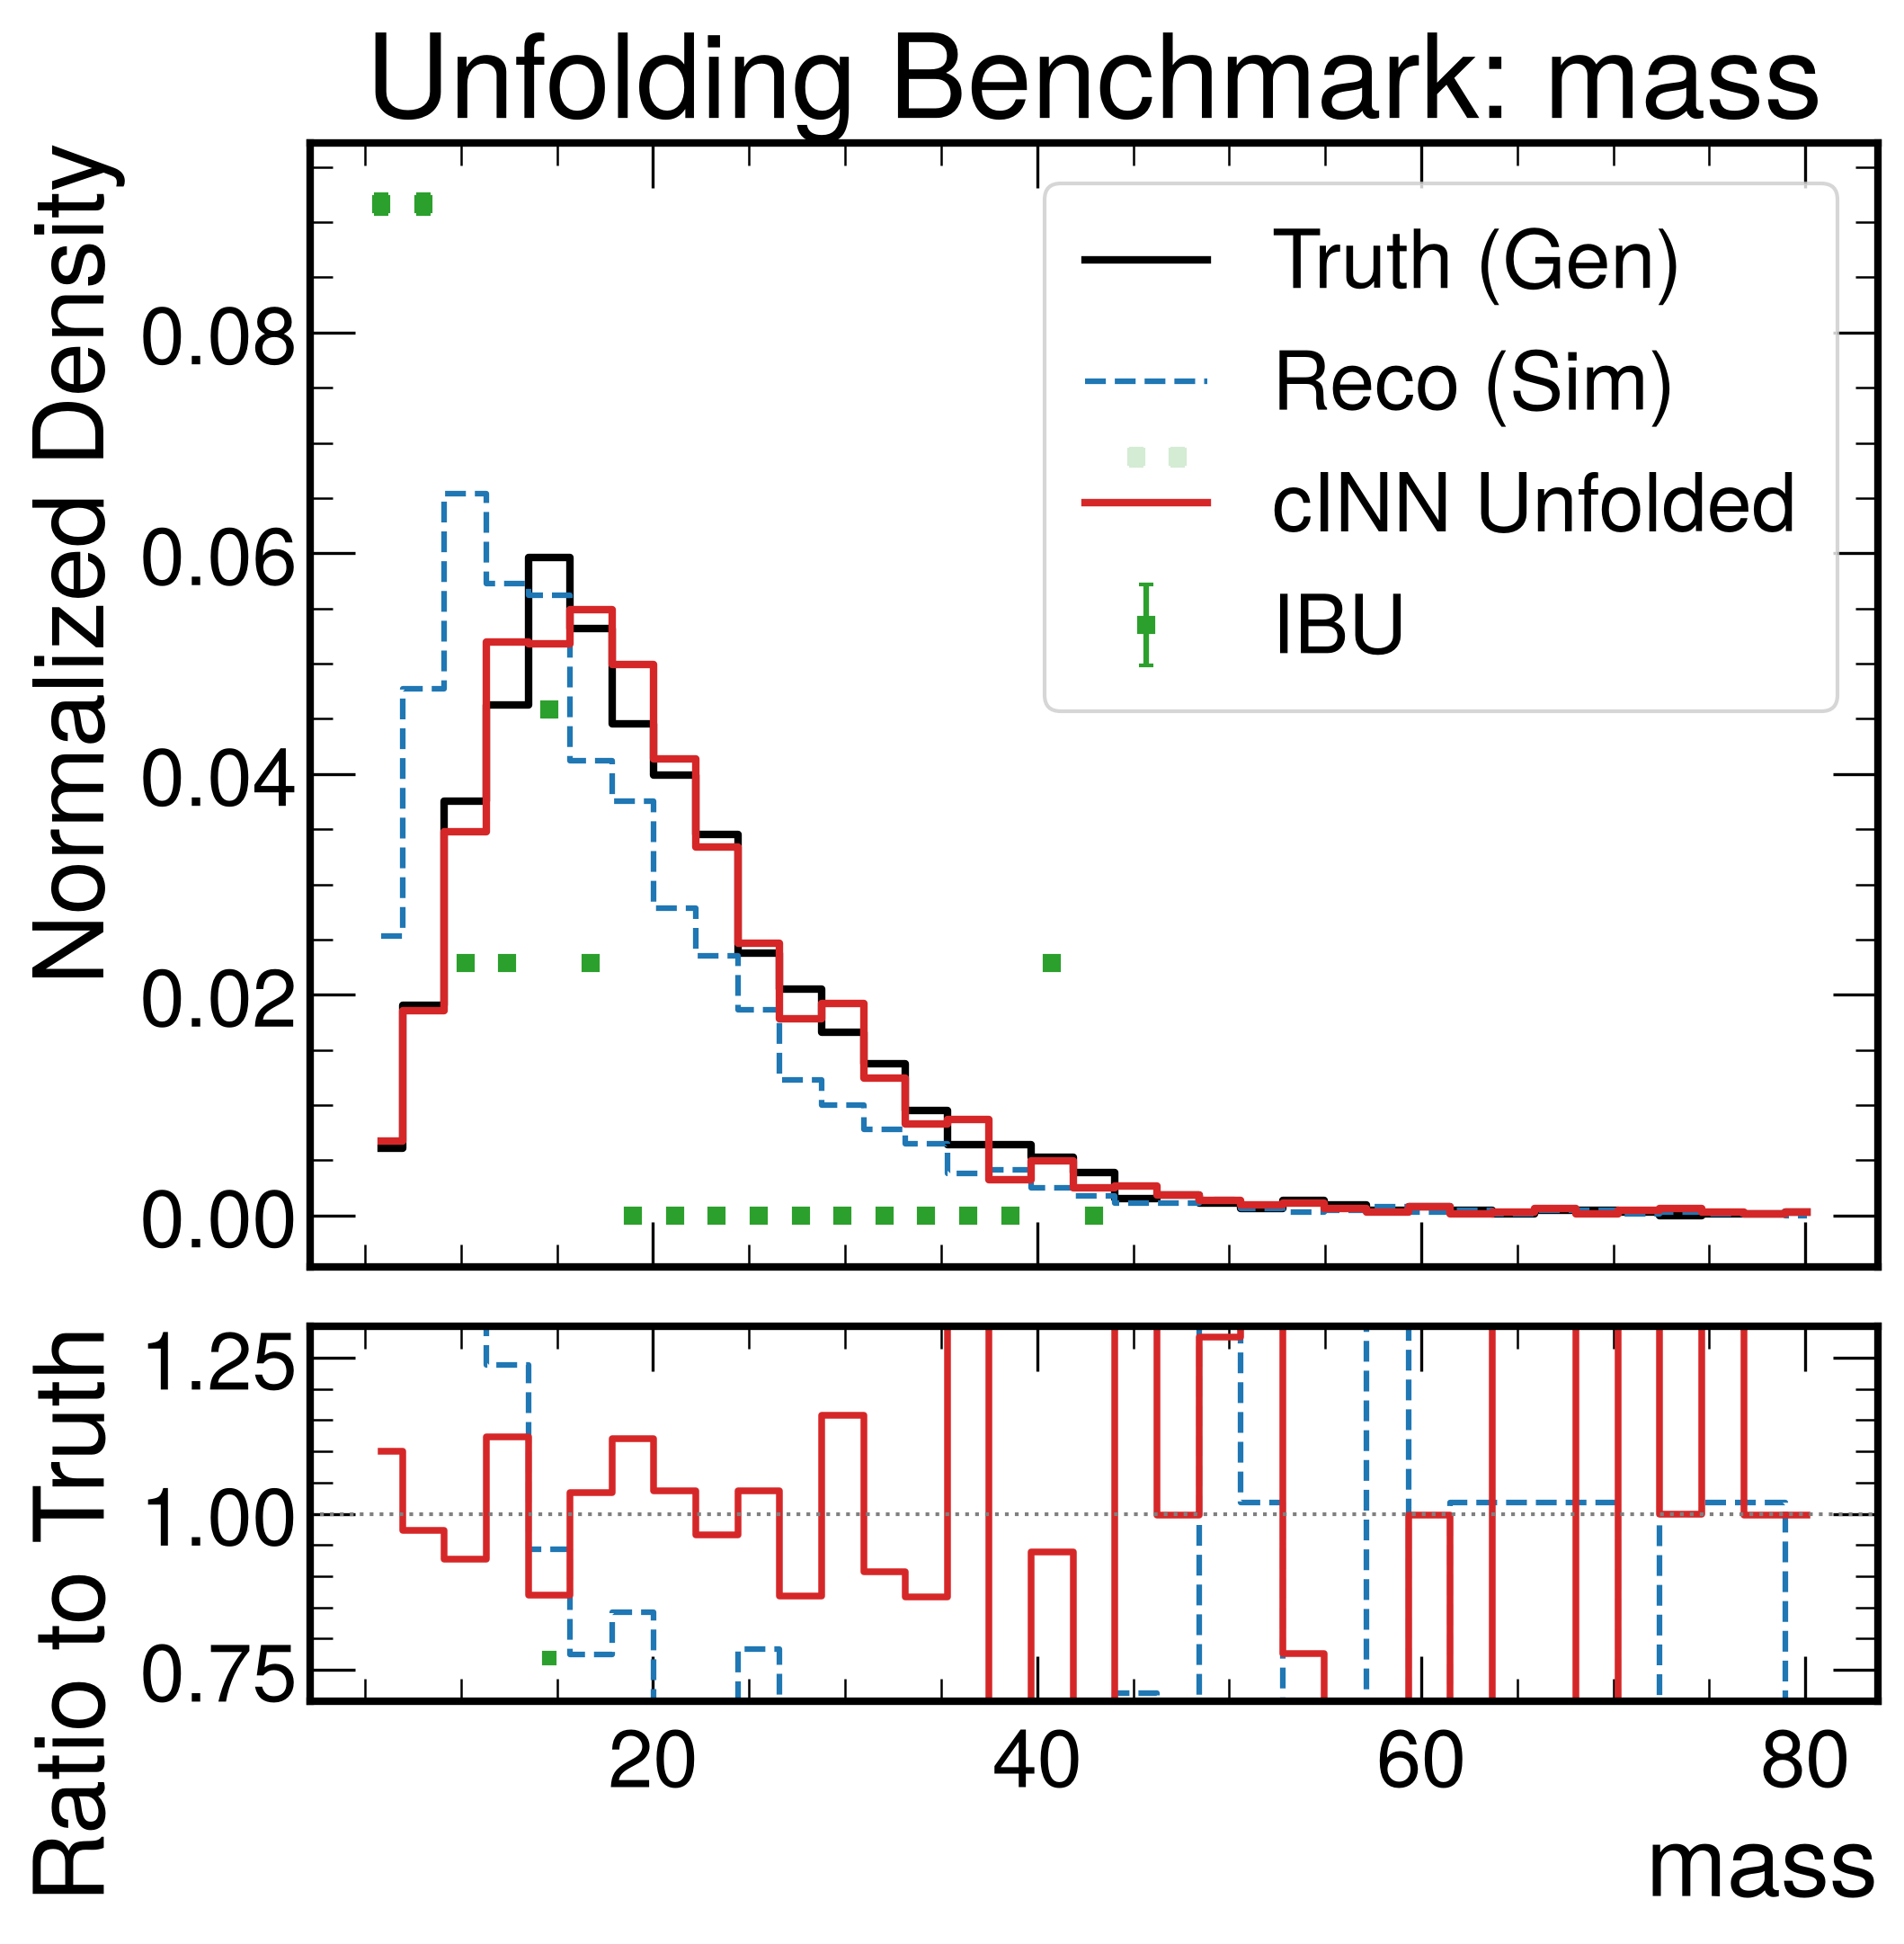
\includegraphics[width=0.88\textwidth]{images/own/benchmark_2d_mass.png}\\
      \tiny\textit{Figure: 2D Jet Mass unfolding comparing Truth (black), Reco (blue), cINN (red), and IBU.}
    \end{column}
  \end{columns}
  \note{To evaluate 1D marginals, we use the Wasserstein-1 Earth Mover's distance and Kolmogorov-Smirnov statistics. In the figure on the right, you can see how detector smearing in blue severely flattens the jet mass distribution. The red cINN curve accurately recovers the black truth spectrum, reducing the Wasserstein distance by over 90 percent and matching or beating classical IBU across both core and tail bins.}
\end{frame}

% -------------------------------------------------------------
% Slide 7: Conditional Correctness & Validation Gates
% -------------------------------------------------------------
\begin{frame}{6. Metrics (2/2): Multidimensional Conditional Gates}
  \begin{columns}[T]
    \begin{column}{0.50\textwidth}
      \begin{itemize}
        \item \textbf{Pair-C2ST Gate:} LightGBM trained on $[x, y]$ pairs.
          \begin{itemize}\footnotesize
            \item Calibrated empirical null: $\mu_{\text{null}} \pm 2\sigma_{\text{null}}$.
            \item \textbf{Pass Rule:} $\text{AUC}_{\text{model}} \le \mu_{\text{null}} + 2\sigma_{\text{null}}$.
            \item 6D cINN achieves \textbf{\pairAUCSixD} (PASS).
          \end{itemize}
        \item \textbf{Negative Control Flow $p(x)$:}
          Unconditional model fails with $\text{AUC} = \mathbf{\controlAUCSixD}$.
        \item \textbf{Simulation-Based Calibration (SBC):}
          Uniform rank histograms confirm posterior accuracy.
      \end{itemize}
    \end{column}
    \begin{column}{0.48\textwidth}
      \centering
      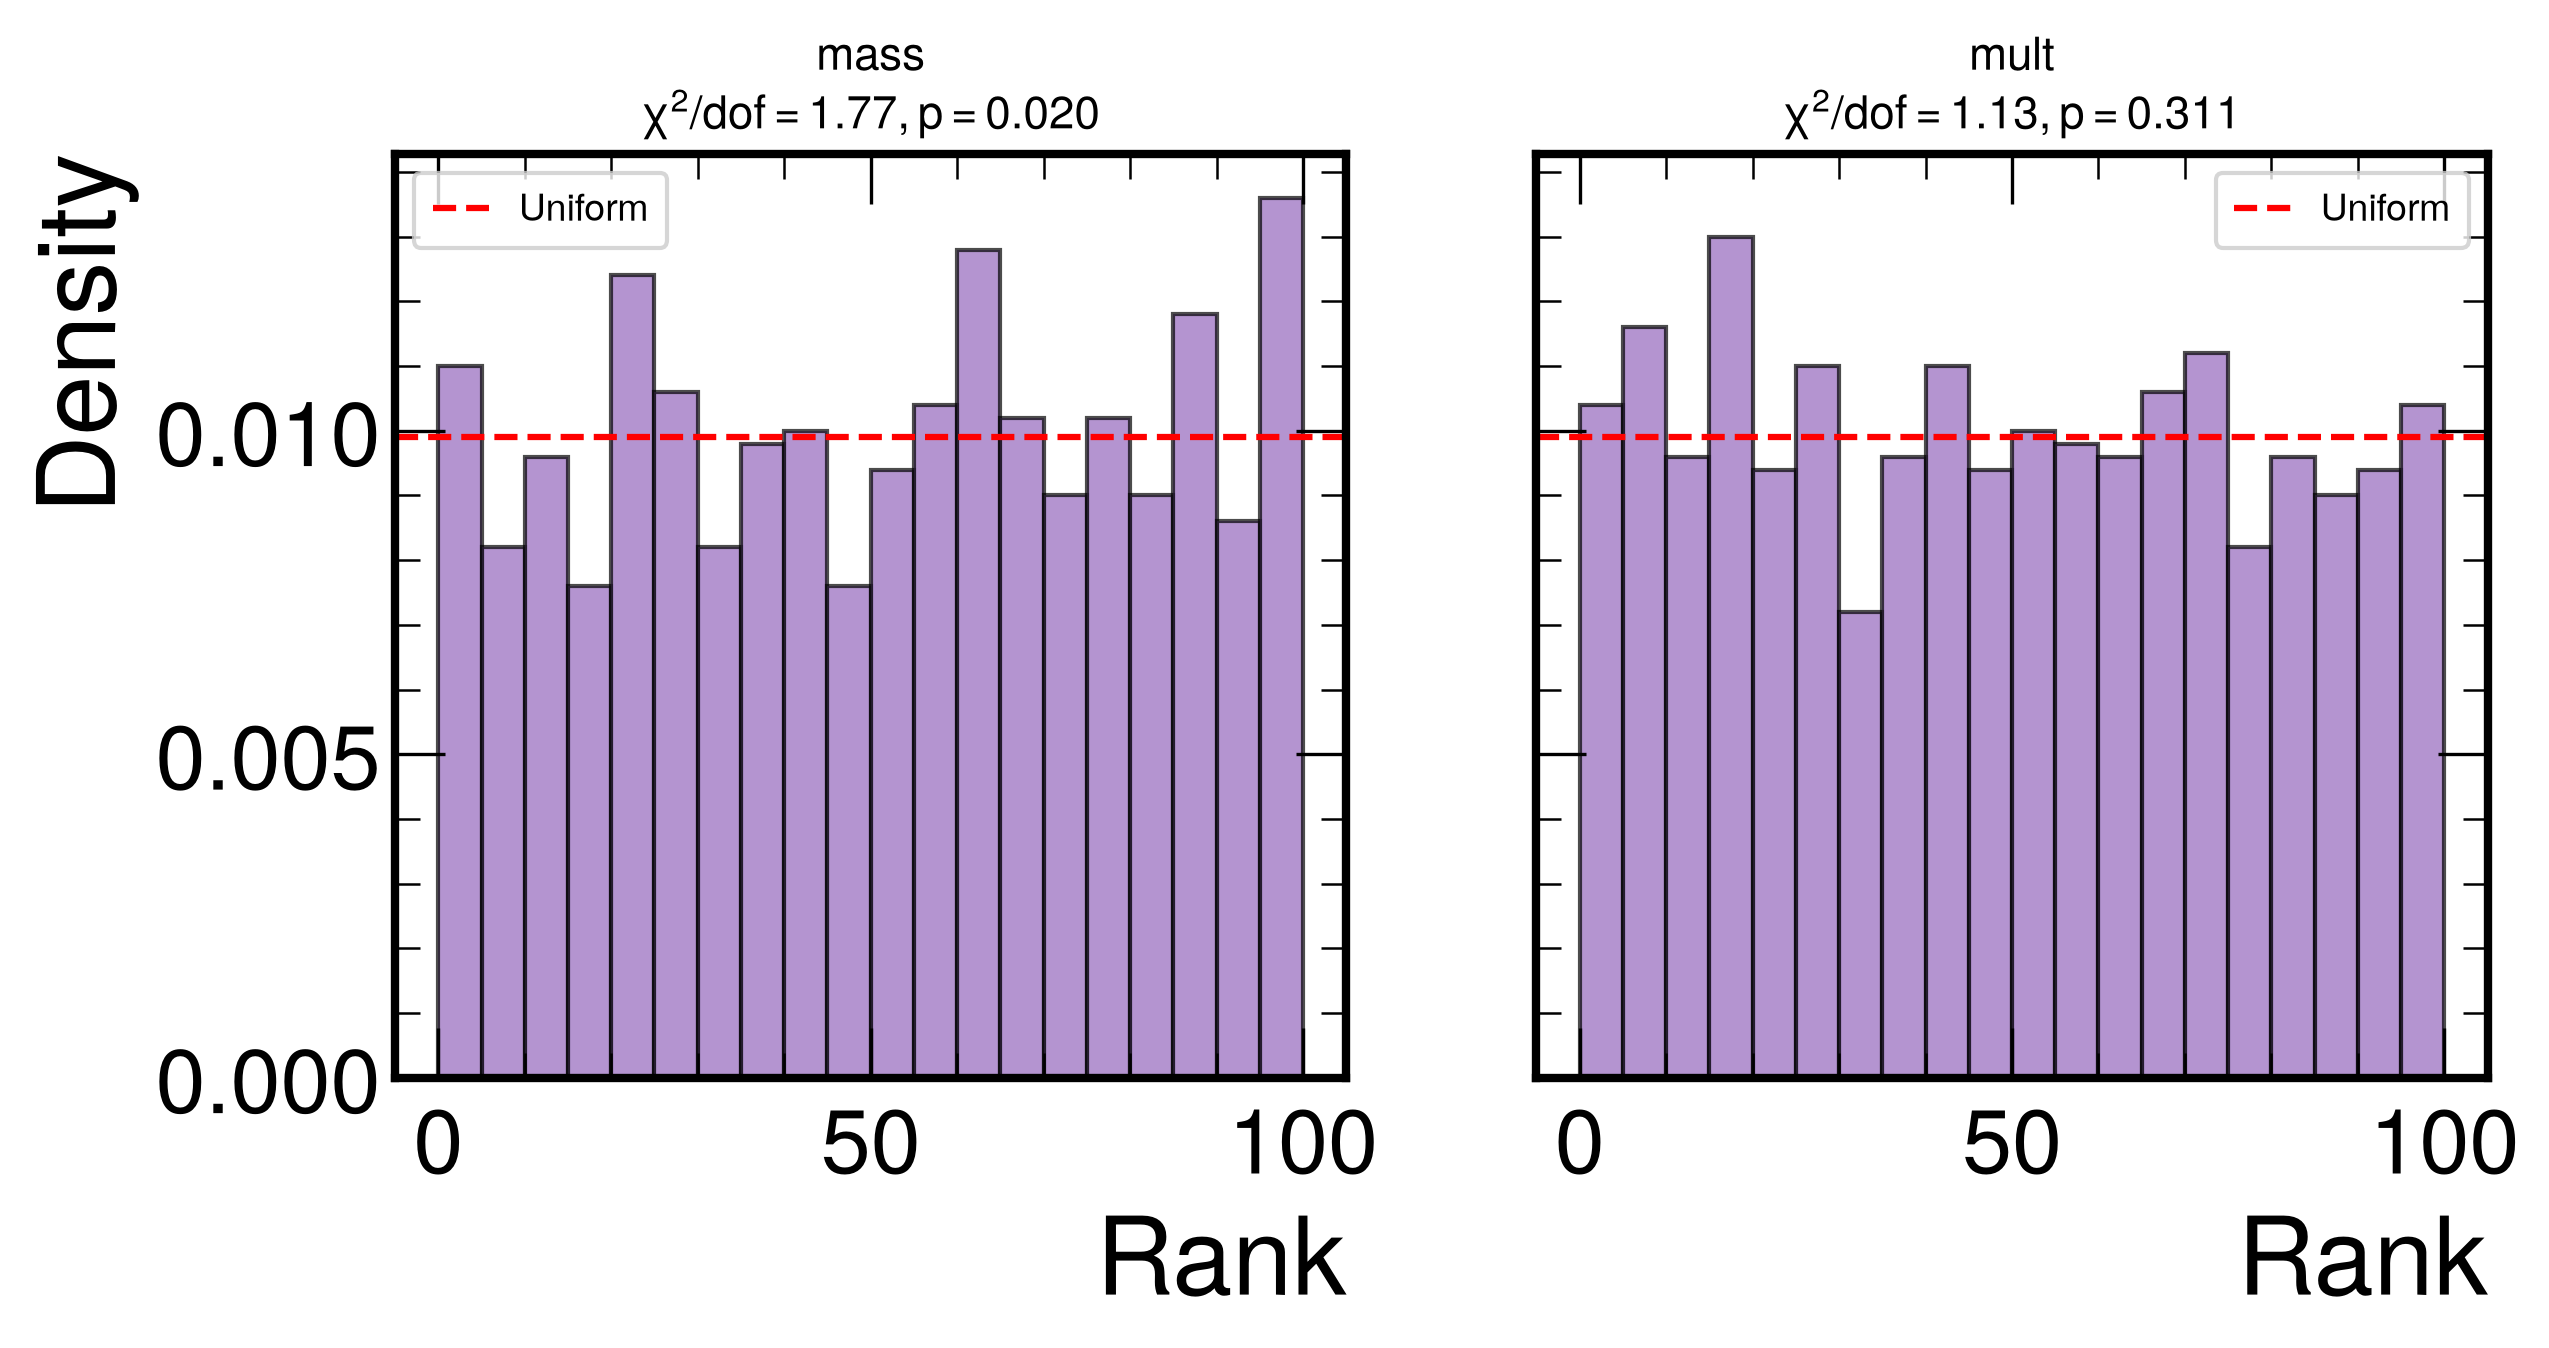
\includegraphics[width=0.88\textwidth]{images/own/sbc_ranks_2d.png}\\
      \tiny\textit{Figure: SBC rank histograms confirming posterior uniformity ($p_{\text{mass}}=0.020, p_{\text{mult}}=0.311$).}
    \end{column}
  \end{columns}
  \note{For multidimensional validation, visual inspection is insufficient. We implement Classifier Two-Sample Tests on joint pairs of truth and detector conditioning. Our 6D cINN achieves a C2ST AUC of 0.45, comfortably passing the null gate. Meanwhile, our negative control model with no conditioning scores 0.90, proving our test reliably detects conditioning. Simulation-Based Calibration ranks shown on the right confirm that posterior uncertainties are well-calibrated.}
\end{frame}

% -------------------------------------------------------------
% Slide 8: Results at a Glance
% -------------------------------------------------------------
\begin{frame}{7. Results Benchmark Across Pythia and Herwig}
  \begin{table}[htbp]
\centering
\footnotesize
\begin{tabular}{lccccc}
\toprule
\textbf{Method} & \textbf{Pythia $W_1$ ($m$/$M$)} & \textbf{Pythia KS ($m$/$M$)} & \textbf{Pair-C2ST AUC} & \textbf{Herwig $W_1$ ($m$/$M$)} & \textbf{Herwig KS ($m$/$M$)} \\
\midrule
Reco-as-answer & 3.60 / 7.09 & 0.208 / 0.329 & -- & 2.33 / 7.50 & 0.115 / 0.294 \\
Prior-only & 0.443 / 0.722 & 0.034 / 0.036 & 0.818 [Fail] & 1.14 / 2.55 & 0.055 / 0.098 \\
IBU (2D) & 0.412 / 0.589 & 0.028 / 0.031 & -- & 1.25 / 2.81 & 0.062 / 0.112 \\
\textbf{cINN 2D (Ours)} & \textbf{0.289 / 0.216} & \textbf{0.021 / 0.016} & \textbf{0.4231 $\pm$ 0.0109 [PASS]} & \textbf{0.85 / 0.20} & \textbf{0.055 / 0.010} \\
\textbf{cINN 6D (Ours)} & \textbf{0.302 / 0.223} & \textbf{0.018 / 0.016} & \textbf{0.4502 $\pm$ 0.0192 [PASS]} & \textbf{0.70 / 0.25} & \textbf{0.044 / 0.017} \\
\bottomrule
\end{tabular}
\end{table}

  \vspace{0.2cm}
  \begin{itemize}\small
    \item \textbf{Pythia Closure:} cINN achieves near-ideal closure; Pair-C2ST confirms indistinguishability.
    \item \textbf{Herwig Stress Test:} Multiplicity detector bias reduced from $-7.50$ to $+0.04$ counts.
    \item \textbf{Scalability:} cINN unfolds all 6 continuous dimensions without histogram binning.
  \end{itemize}
  \note{This table summarizes the overall benchmarking. On Pythia nominal testing, cINN achieves state-of-the-art closure across both 2D and 6D targets. Crucially, on out-of-distribution Herwig events, while raw detector reconstruction carries a severe negative 7.5 count bias in multiplicity, the cINN restores it to within 0.04 counts. Classical IBU fails to scale beyond 2D, while cINN handles the full 6-observable phase space seamlessly.}
\end{frame}

% -------------------------------------------------------------
% Slide 9: Outputs and Deliverables
% -------------------------------------------------------------
\begin{frame}{8. Outputs, Deliverables \& Workload Split}
  \begin{columns}[T]
    \begin{column}{0.50\textwidth}
      \begin{itemize}
        \item \textbf{Codebase Deliverables:}
          \begin{itemize}\footnotesize
            \item Modular package in \texttt{src/unfold/}
            \item Automated pipeline: \texttt{make all}
            \item 14 automated unit tests in \texttt{pytest}
            \item 12 flow checkpoints across 3 seeds
            \item Technical reports and project report PDF
          \end{itemize}
        \item \textbf{Workload Split (Option C):}
          \begin{itemize}\footnotesize
            \item \textbf{Alfien Jessurun P:} cINN Zuko RQ-NSF architecture, context embedding MLP, invertible transforms with analytical Jacobians, multi-seed training loops.
            \item \textbf{Boopesh D:} Delphes data ingestion, D'Agostini IBU baseline, LightGBM Pair-C2ST null gates, SBC calibration, Herwig stress tests.
          \end{itemize}
      \end{itemize}
    \end{column}
    \begin{column}{0.48\textwidth}
      \centering
      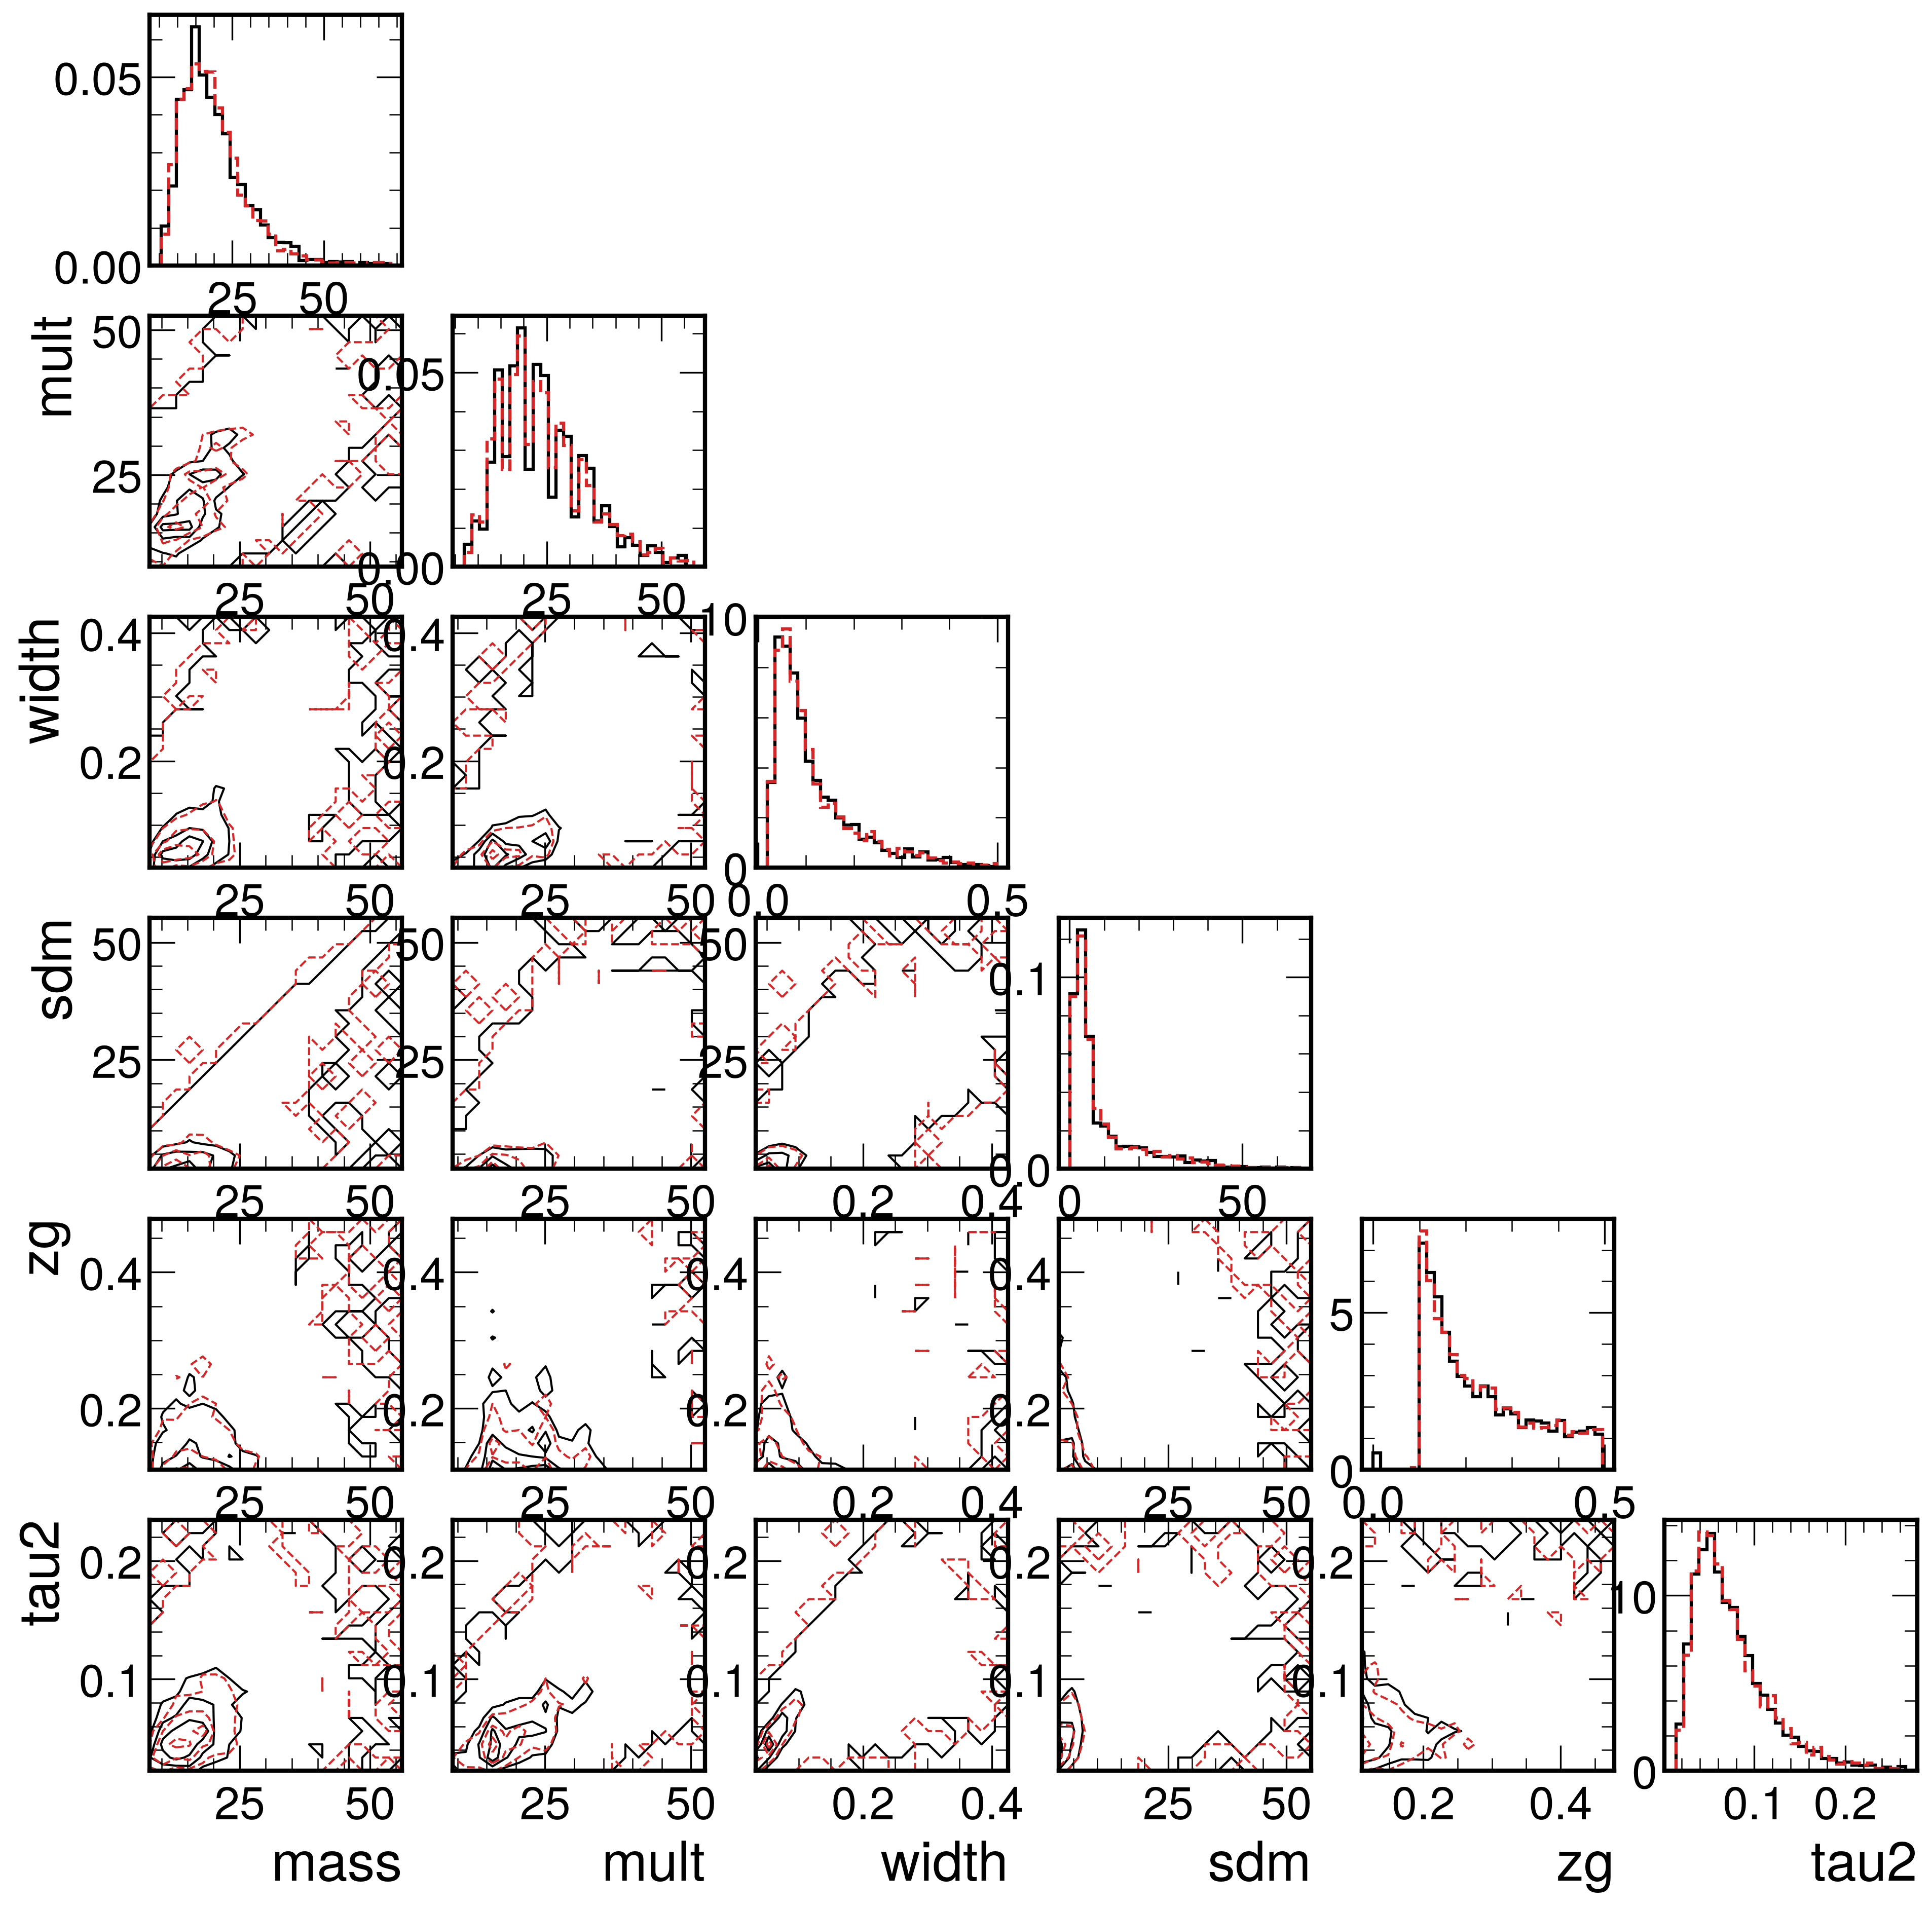
\includegraphics[width=0.90\textwidth]{images/own/corner_6d_pairwise.png}\\
      \tiny\textit{Figure: 15-pairwise corner correlation matrix across 6 substructure observables.}
    \end{column}
  \end{columns}
  \note{To conclude, the project produced a fully automated, reproducible codebase complete with unit tests, multi-seed checkpoints, and full documentation. Work was divided cleanly under Option C, with Alfien leading core flow architecture and invertible transforms, and Boopesh leading data pipeline ingestion, IBU baselines, and statistical validation. On the right is our 15-pairwise 6D correlation plot capturing the full non-linear jet substructure.}
\end{frame}

% -------------------------------------------------------------
% Slide 10: Image Credits Frame
% -------------------------------------------------------------
\begin{frame}[noframenumbering]{Image Credits \& Citations}
  \footnotesize
  \begin{itemize}
    \item \textbf{Benchmark Results Figures (Slides 6, 7, 8, 9):} Generated directly from project execution scripts and raw Delphes simulation data; authored by Alfien Jessurun P and Boopesh D.
    \item \textbf{CMS Detector Reference (Slide 2):} CERN / CMS Collaboration, CERN Document Server, CC-BY-4.0.
    \item \textbf{Methodology \& Architecture References:}
      \begin{itemize}\scriptsize
        \item A. Andreassen et al., \textit{OmniFold: A Method to Simultaneously Unfold All Observables}, PRL 124, 112002 (2020).
        \item A. Backes et al., \textit{Unbinned Detector Unfolding with Conditional Invertible Neural Networks}, SciPost Phys. Core 6, 065 (2023).
        \item C. Durkan et al., \textit{Neural Spline Flows}, NeurIPS 32 (2019).
      \end{itemize}
  \end{itemize}
\end{frame}

% -------------------------------------------------------------
% Slide 11: Dedicated Thank You Slide
% -------------------------------------------------------------
\begin{frame}[noframenumbering]
  \centering
  \vspace{1.5cm}
  {\Huge\textbf{\textcolor{IITHorange}{Thank You!}}}
  \par\vspace{0.5cm}
  {\large Questions \& Discussion}
  \par\vspace{0.8cm}
  \textbf{Alfien Jessurun P} (\texttt{ep23btech11001@iith.ac.in})\\
  \textbf{Boopesh D} (\texttt{ep23btech11007@iith.ac.in})\\
  \vspace{0.2cm}
  \footnotesize Department of Physics, Indian Institute of Technology Hyderabad
\end{frame}

\end{document}
